\section{Рекомендации по оформлению работы}

Этот раздел содержит рекомендации по оформлению пояснительной записки
и примеры использования различных \LaTeX-конструкций. При подготовке
реального отчёта о выполненной работе данный раздел, естественно, должен
быть опущен.

\subsection*{Общие замечания по структуре курсовой работы}

Обычно в любой работе должно быть \emph{не менее} трёх разделов. Приложение
(или приложения) с текстами программ \emph{не должны} составлять б\'{о}льшую
часть работы. Хорошо, когда в работе имеются таблицы, рисунки или диаграммы,
«снимки экрана» и математические формулы. Возможна, например, такая 
структура работы:

\begin{itemize}
\item введение, содержащее постановку решаемой задачи (или задач);
\item изложение необходимых для решения задачи теоретических аспектов;
\item описание используемых структур данных и применяемых алгоритмов;
\item возможные обобщения рассматриваемой задачи;
\item приложения с фрагментами программ;
\item список литературы и интернет-ресурсов.
\end{itemize}

\subsection*{Рекомендации по использованию \LaTeX}

Для подготовки пояснительной записки следует применять \LaTeX\ и пакет 
\texttt{memoir}. Настоятельно рекомендуется использовать в исходных 
\TeX-файлах кодировку \texttt{UTF-8}. При этом длина большей части строк в 
этих файлах не должна превосходить 79 символов. Рекомендуется 
использовать только те команды переключения шрифтов, которые поддерживаются
пакетом \verb|memoir| без опции \verb|oldfontcommands|. 

При создании pdf-файла используются головной файл \texttt{paper.tex} и 
стилевой файл \texttt{msiu\_term\_work.sty}, в котором подключаются 
дополнительные 
пакеты, определяются размеры полей, стиль оформления страниц и целый ряд иных 
параметров и макросов, включая макрос, задающий титульный лист пояснительной
записки. В компьютерных классах МГИУ стилевой файл постоянно обновляется,
поэтому при подготовке пояснительной записки на домашнем компьютере необходимо
использовать последнюю версию этого файла.

При наборе русского текста перед знаками препинания пробел не ставится, 
а после них~--- ставится всегда. Следует использовать букву «ё», 
кавычки-ёлочки 
(например, \verb|«Информационные технологии и моделирование»|) и
прямой шрифт при наборе единиц измерения (кг, м/сек${}^2$).
При записи инициалов людей рекомендуется применять «сверхтонкий пробел» 
(\verb|\+|) между именем и отчеством и «неразрывный пробел» (\verb|~|) между
отчеством и фамилией: \verb|И.\+И.~Иванов|. 

Следует использовать по назначению тире
(---), «указатель диапазона» (--), дефис (-) и математический знак «минус»
($-$). Перед тире рекомендуется ставить «неразрывный
пробел», а после него~--- обычный: \verb|после него~--- обычный|. Указатель
диапазона применяется, например, при указании страниц: стр. 15--17
(набирается как \verb|стр. 15--17|). Для набора дефиса необходим минус: 
\verb|объектно-ориентированный|, а для получения знака операции  «минус»
требуется применять математический режим: число $-2$ набирается как
\verb|$-2$|. 

Сокращения словосочетаний «и так далее» и «и тому подобное», которые
завершают предложение, набираются так: \verb|и~т.\,д.|, \verb|и~т.\,п.|
Не рекомендуется использовать подобные сокращения для словосочетаний,
находящихся в середине предложения. Для набора нумерованных списков 
целесообразно использовать окружение \verb|\enumerate| в~следующем виде:
\verb|\begin{enumerate}[1)]|.
Стандартный стиль оформления рисунков и таблиц~--- использование окружений
\verb|figure| и \verb|table|. При этом обязательно следует применять макрос
\verb|caption| для набора подписи. 

При наборе математических формул следует нумеровать только те из них, на
которые имеются ссылки. Для получения полужирного шрифта в математических
формулах можно применять команду \verb|\bm|: $\pi \ne \bm\pi$.

О наборе математики мы уже говорили весьма подробно, поэтому сейчас 
ограничимся лишь двумя примерами. Следующий код
\begin{small}
\begin{verbatim}
$$\int\limits_a^b\frac12 (1+x)^{-3/2}dx=
\left.-\frac{1}{\sqrt{1+x}}\right|_a^b$$
\end{verbatim}
\end{small}
\noindent позволяет получить формулу

$$\int\limits_a^b\frac12 (1+x)^{-3/2}dx=
\left.-\frac{1}{\sqrt{1+x}}\right|_a^b$$

Приведённый ниже фрагмент кода из книги~\cite{roganov-jurists}
является более сложным.
\begin{small}
\begin{verbatim}
Рассмотрим сначала одну из самых простых функций~$y=x^{2}$. Обычно правую
часть в аналитической записи функции обозначают через $f(x)$. Итак, у нас
$f(x)=x^{2}$. Заметим, что значение этой функции в точке $x_{0} = 2$ равно
$y_{0} = 4$, и возьмём на оси $X$ бесконечную последовательность точек с
координатами $x_{n}=2-1/2^{n - 1}$: $x_{1}=2-1=1$; $x_{2}=2-1/2=3/2$;
$x_{3}=2-1/4=1 3/4$; $\ldots$

\noindent
Эта последовательность, как мы выяснили в \S1, имеет предел, равный двум:
$\displaystyle\lim_{n \to \infty } x_n = 2$. Найдём значения функции
$f(x)$ в выбранных точках: 
$$\displaylines{
y_1=f(x_1)=f(1)=1;\cr
y_2=f(x_2)=f\left(\dfrac32\right)= \dfrac94;\cr
y_3=f(x_3)=f\left(\dfrac74\right)=\dfrac{49}{16};\cr
\ldots\ldots\ldots\ldots\ldots\ldots\ldots\ldots\ldots;\cr
y_n=f(x_n)=f\left(2-\dfrac{1}{2^{n-1}}\right)=
\left(2-\dfrac{1}{2^{n-1}}\right)^2=4-\dfrac{1}{2^{n-3}}+\dfrac{1}{2^{2n-2}}.
}$$
\end{verbatim}
\end{small}
\noindent Вот во что он превращается:

Рассмотрим сначала одну из самых простых функций~$y=x^{2}$. Обычно правую
часть в аналитической записи функции обозначают через $f(x)$. Итак, у нас
$f(x)=x^{2}$. Заметим, что значение этой функции в точке $x_{0} = 2$ равно
$y_{0} = 4$, и возьмём на оси $X$ бесконечную последовательность точек с
координатами $x_{n}=2-1/2^{n - 1}$: $x_{1}=2-1=1$; $x_{2}=2-1/2=3/2$;
$x_{3}=2-1/4=1 3/4$; $\ldots$

\noindent
Эта последовательность, как мы выяснили в \S1, имеет предел, равный двум:
$\displaystyle\lim_{n \to \infty } x_n = 2$. Найдём значения функции
$f(x)$ в выбранных точках: 
$$\displaylines{
y_1=f(x_1)=f(1)=1;\cr
y_2=f(x_2)=f\left(\dfrac32\right)= \dfrac94;\cr
y_3=f(x_3)=f\left(\dfrac74\right)=\dfrac{49}{16};\cr
\ldots\ldots\ldots\ldots\ldots\ldots\ldots\ldots\ldots;\cr
y_n=f(x_n)=f\left(2-\dfrac{1}{2^{n-1}}\right)=
\left(2-\dfrac{1}{2^{n-1}}\right)^2=4-\dfrac{1}{2^{n-3}}+\dfrac{1}{2^{2n-2}}.
}$$

Теперь рассмотрим пример простой таблицы, которая строится с помощью окружения
\verb|tabular|, и состоит из трёх столбцов. Содержимое каждого столбца может
центрироваться (\verb|c|), либо прижиматься к левому (\verb|l|) или правому
(\verb|r|) краям. Символ~\verb|&| указывает на границу между столбцами, а
символы \verb|\\| --- на конец строки таблицы. Следует понимать, что в таблице 
вовсе не обязаны присутствовать горизонтальные и вертикальные линии. Вот как
можно задать грамматику, используя именно такую таблицу:

\medskip
\noindent\hspace{2cm}
\begin{tabular}{rll}
$\alpha \rightarrow$ & $ab\beta$\\
$\beta  \rightarrow$ & $\alpha\mid\gamma$\\
$\gamma \rightarrow$ & $\beta\mid\varepsilon$\\
\end{tabular}
\medskip

\noindent Исходный код для получения этой таблицы имеет следующий вид:

\begin{small}
\begin{verbatim}
\noindent\hspace{2cm}
\begin{tabular}{rll}
$\alpha \rightarrow$ & $ab\beta$\\
$\beta  \rightarrow$ & $\alpha\mid\gamma$\\
$\gamma \rightarrow$ & $\beta\mid\varepsilon$\\
\end{tabular}
\end{verbatim}
\end{small}

Более сложной является таблица~\ref{tabl:crayfish}, позаимствованная из книги
С.\+М.~Львовского~\cite{rlatex}. Заметим, что эта таблица снабжена
подписью (caption) и меткой (label), позволяющей ссылаться на неё.

\begin{table}[ht!]
\caption{Известная шутка М.\+М.~Жванецкого}\label{tabl:crayfish}
\begin{center}
\begin{tabular}{|p{5cm}|p{5cm}|}
\hline
\multicolumn{2}{|c|}{\large\textbf{Я видел раков}}\\
\hline
Вчера: & Сегодня: \\
\hline
Маленькие, но по три рубля, но очень
маленькие, но по три, но очень маленькие.
&
Большие, но по пять рублей, но большие, но
по пять рублей, но очень большие,
но по пять.\\
\hline
\end{tabular}
\end{center}
\end{table}

\noindent 
Вот каков исходный код таблицы~\ref{tabl:crayfish}:

\begin{small}
\begin{verbatim}
\begin{table}[ht!]
\caption{Известная шутка М.\+М.~Жванецкого}\label{tabl:crayfish}
\begin{center}
\begin{tabular}{|p{5cm}|p{5cm}|}
\hline
\multicolumn{2}{|c|}{\large\textbf{Я видел раков}}\\
\hline
Вчера: & Сегодня: \\
\hline
Маленькие, но по три рубля, но очень
маленькие, но по три, но очень маленькие.
&
Большие, но по пять рублей, но большие, но
по пять рублей, но очень большие,
но по пять.\\
\hline
\end{tabular}
\end{center}
\end{table}
\end{verbatim}
\end{small}

Наиболее правильным вариантом включение изображения (формата \verb|png| или
\verb|jpg|)
в документ является использование окружения \verb|figure|, что
даёт возможность использовать подписи и нумеровать рисунки.

\begin{figure}[ht!]
\begin{center}

\includegraphics[scale=0.6]{images/msiu_logo}
\end{center}
\vspace*{-8mm}
\caption{Логотип МГИУ}\label{fig:msiu_logo}
\end{figure}

\newpage

Исходный код, использованный для включения логотипа МГИУ,
изображённого на рис.~\ref{fig:msiu_logo}, таков:

\begin{small}
\begin{verbatim}
\begin{figure}[ht!]
\begin{center}

\includegraphics[scale=0.6]{images/msiu_logo}
\end{center}
\vspace*{-8mm}
\caption{Логотип МГИУ}\label{fig:msiu_logo}
\end{figure}
\end{verbatim}
\end{small}

Часто бывает полезно включать в документ «снимки экрана», масштабируя
картинку нужным образом. Примером является рис.~\ref{fig:rating}.

\begin{figure}[ht!]
\begin{center}
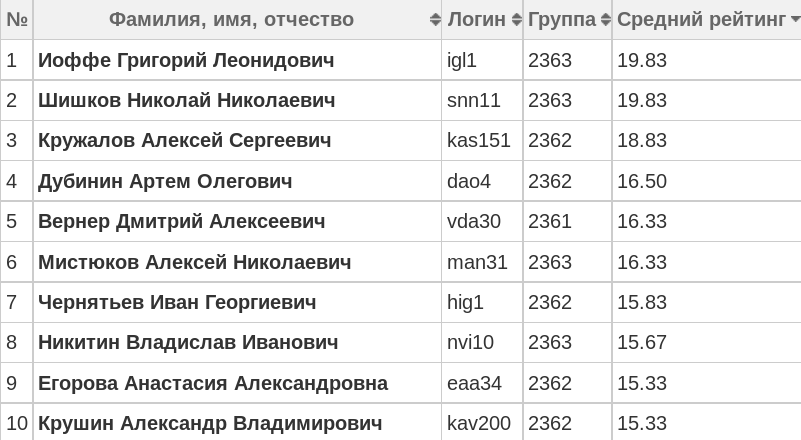
\includegraphics[width=0.85\hsize]{images/rating}
\end{center}
\caption{Рейтинг}\label{fig:rating}
\end{figure}

Иногда можно воспользоваться возможностями самого \LaTeX'а,
позволяющего создавать «псевдорисунки». Вот исходный код
рис.~\ref{fig:simple}:

\begin{small}
\begin{verbatim}
\begin{picture}(120,80)
% Границы изображения:
\put(0,0){\line(1,0){120}}
\put(0,80){\line(1,0){120}}
\put(0,0){\line(0,1){80}}
\put(120,0){\line(0,1){80}}
%
% Оси координат:
\put(40,25){\begin{picture}(40,40)%
              \put(20,0){\vector(0,1){40}}
              \put(0,20){\vector(1,0){40}}
              \put(40,22){$x$}
              \put(22,40){$y$}
            \end{picture}}
\end{picture}
\end{verbatim}
\end{small}

\begin{figure}[ht!]
\begin{center}
\begin{picture}(120,80)
% Границы изображения:
\put(0,0){\line(1,0){120}}
\put(0,80){\line(1,0){120}}
\put(0,0){\line(0,1){80}}
\put(120,0){\line(0,1){80}}
%
% Оси координат:
\put(40,25){\begin{picture}(40,40)%
              \put(20,0){\vector(0,1){40}}
              \put(0,20){\vector(1,0){40}}
              \put(40,22){$x$}
              \put(22,40){$y$}
            \end{picture}}
\end{picture}
\end{center}
\caption{Простой псевдорисунок}\label{fig:simple}
\end{figure}

Гораздо более интересным является рис~\ref{fig:cos_acos}, 
исходный код для которого создан с помощью небольшого скрипта,
написанного на языке Ruby и приведённого в приложении.

\begin{figure}[ht!]
\begin{center}
% Цвет для клеточек
\definecolor{gridcolor}{cmyk}{0.30,0.00,0.0,0.0}
% Основной цвет гистограмм и графиков
\definecolor{plot1}{cmyk}{0.9,0.5,0.0,0.0} 
% Второй цвет гистограмм и графиков
\definecolor{plot2}{cmyk}{0.0,0.60,0.70,0.0} 
% Толщина линии у клеточек
\newlength\gridwidth
\setlength{\gridwidth}{0.8pt}
% Макрос для включения клеточек
\newcommand{\mygrid}[4]{
\begin{pgfscope}
\pgfsetlinewidth{\gridwidth}\color{gridcolor}
\pgfgrid[stepx=0.5cm,stepy=0.5cm]{\pgfxy(#1,#2)}{\pgfxy(#3,#4)}
\end{pgfscope}
}
% Толщина линии у графиков
\newlength\plotwidth
\setlength{\plotwidth}{1.2pt}

% Собственно картинка
\begin{pgfpicture}{0mm}{0mm}{ 69.333mm}{ 69.333mm}
\pgfsetxvec{\pgfpoint{  8.000mm}{0mm}}
\pgfsetyvec{\pgfpoint{0mm}{  8.000mm}}
\begin{pgftranslate}{\pgfpoint{ 34.667mm}{ 34.667mm}}
%
\mygrid{-4.2}{-4.2}{4.2}{4.2}
%
\pgfsetendarrow{\pgfarrowsingle}
\pgfxyline( -4.333,0)(  4.333,0)
\pgfxyline(0, -4.333)(0,  4.333)
\pgfclearendarrow
%
\pgfputat{\pgfxy( 0.400, -0.480)}{\pgfbox[right,base]{\small$O$}}
\pgfputat{\pgfxy(  4.333, -0.480)}{\pgfbox[right,base]{\small $X$}}
\pgfputat{\pgfxy( -0.100,  4.333)}{\pgfbox[right,top]{\small $Y$}}
%
\pgfxyline(1, -0.100)(1,  0.100)
\pgfputat{\pgfxy(  1, -0.480)}{\pgfbox[center,base]{\small $1$}}
\pgfxyline(-1, -0.100)(-1,  0.100)
\pgfputat{\pgfxy(  -1.000, -0.480)}{\pgfbox[center,base]{\small $-1$}}
\pgfxyline(3.1416, -0.100)(3.1416,  0.100)
\pgfputat{\pgfxy(  3.1416, 0.280)}{\pgfbox[center,base]{\small $\pi$}}
\pgfxyline( -0.100,3.1416)(  0.100,3.1416)
\pgfputat{\pgfxy( 0.400,  3.1416)}{\pgfbox[right,center]{\small $\pi$}}
%
\pgfsetdash{{0.1cm}{0.1cm}}{0cm}
\pgfxyline(3.1416, 0)(3.1416, -1.0)
\pgfxyline(-1,3.1416)(0,3.1416)
\pgfsetdash{}{0cm}
%
\pgfsetdash{{0.2cm}{0.1cm}}{0cm}
\pgfxyline(-1,-1)(3,3)
\pgfsetdash{}{0cm}
%
\color{plot1}
\pgfxycurve( -4.333, -0.370)( -4.222, -0.473)( -4.111, -0.570)( -4.000, -0.654)
\pgfxycurve( -4.000, -0.654)( -3.889, -0.738)( -3.778, -0.810)( -3.667, -0.865)
\pgfxycurve( -3.667, -0.865)( -3.556, -0.921)( -3.444, -0.960)( -3.333, -0.982)
\pgfxycurve( -3.333, -0.982)( -3.222, -1.003)( -3.111, -1.006)( -3.000, -0.990)
\pgfxycurve( -3.000, -0.990)( -2.889, -0.974)( -2.778, -0.940)( -2.667, -0.889)
\pgfxycurve( -2.667, -0.889)( -2.556, -0.839)( -2.444, -0.771)( -2.333, -0.691)
\pgfxycurve( -2.333, -0.691)( -2.222, -0.610)( -2.111, -0.517)( -2.000, -0.416)
\pgfxycurve( -2.000, -0.416)( -1.889, -0.315)( -1.778, -0.206)( -1.667, -0.096)
\pgfxycurve( -1.667, -0.096)( -1.556,  0.015)( -1.444,  0.127)( -1.333,  0.235)
\pgfxycurve( -1.333,  0.235)( -1.222,  0.343)( -1.111,  0.447)( -1.000,  0.540)
\pgfxycurve( -1.000,  0.540)( -0.889,  0.634)( -0.778,  0.717)( -0.667,  0.786)
\pgfxycurve( -0.667,  0.786)( -0.556,  0.855)( -0.444,  0.909)( -0.333,  0.945)
\pgfxycurve( -0.333,  0.945)( -0.222,  0.981)( -0.111,  1.000)( -0.000,  1.000)
\pgfxycurve( -0.000,  1.000)(  0.111,  1.000)(  0.222,  0.981)(  0.333,  0.945)
\pgfxycurve(  0.333,  0.945)(  0.444,  0.909)(  0.556,  0.855)(  0.667,  0.786)
\pgfxycurve(  0.667,  0.786)(  0.778,  0.717)(  0.889,  0.634)(  1.000,  0.540)
\pgfxycurve(  1.000,  0.540)(  1.111,  0.447)(  1.222,  0.343)(  1.333,  0.235)
\pgfxycurve(  1.333,  0.235)(  1.444,  0.127)(  1.556,  0.015)(  1.667, -0.096)
\pgfxycurve(  1.667, -0.096)(  1.778, -0.206)(  1.889, -0.315)(  2.000, -0.416)
\pgfxycurve(  2.000, -0.416)(  2.111, -0.517)(  2.222, -0.610)(  2.333, -0.691)
\pgfxycurve(  2.333, -0.691)(  2.444, -0.771)(  2.555, -0.838)(  2.667, -0.889)
\pgfxycurve(  2.667, -0.889)(  2.778, -0.940)(  2.889, -0.974)(  3.000, -0.990)
\pgfxycurve(  3.000, -0.990)(  3.111, -1.006)(  3.222, -1.003)(  3.333, -0.982)
\pgfxycurve(  3.333, -0.982)(  3.444, -0.961)(  3.555, -0.921)(  3.667, -0.865)
\pgfxycurve(  3.667, -0.865)(  3.778, -0.810)(  3.889, -0.738)(  4.000, -0.654)
\pgfxycurve(  4.000, -0.654)(  4.111, -0.570)(  4.222, -0.473)(  4.333, -0.370)
%
\pgfsetlinewidth{\plotwidth}
\pgfxycurve(  0.000,  1.000)(  0.131,  1.000)(  0.263,  0.974)(  0.394,  0.923)
\pgfxycurve(  0.394,  0.923)(  0.526,  0.873)(  0.657,  0.798)(  0.788,  0.705)
\pgfxycurve(  0.788,  0.705)(  0.920,  0.612)(  1.051,  0.500)(  1.183,  0.379)
\pgfxycurve(  1.183,  0.379)(  1.314,  0.257)(  1.445,  0.125)(  1.577, -0.006)
\pgfxycurve(  1.577, -0.006)(  1.708, -0.137)(  1.840, -0.269)(  1.971, -0.390)
\pgfxycurve(  1.971, -0.390)(  2.102, -0.511)(  2.234, -0.621)(  2.365, -0.713)
\pgfxycurve(  2.365, -0.713)(  2.497, -0.806)(  2.628, -0.879)(  2.759, -0.928)
\pgfxycurve(  2.759, -0.928)(  2.891, -0.977)(  3.022, -1.002)(  3.154, -1.000)
%
\color{plot2}
\pgfxycurve(  1.000,  0.000)(  1.000,  0.131)(  0.974,  0.263)(  0.923,  0.394)
\pgfxycurve(  0.923,  0.394)(  0.873,  0.526)(  0.798,  0.657)(  0.705,  0.788)
\pgfxycurve(  0.705,  0.788)(  0.612,  0.920)(  0.500,  1.051)(  0.379,  1.183)
\pgfxycurve(  0.379,  1.183)(  0.257,  1.314)(  0.125,  1.445)( -0.006,  1.577)
\pgfxycurve( -0.006,  1.577)( -0.137,  1.708)( -0.269,  1.840)( -0.390,  1.971)
\pgfxycurve( -0.390,  1.971)( -0.511,  2.102)( -0.621,  2.234)( -0.713,  2.365)
\pgfxycurve( -0.713,  2.365)( -0.806,  2.497)( -0.879,  2.628)( -0.928,  2.759)
\pgfxycurve( -0.928,  2.759)( -0.977,  2.891)( -1.002,  3.022)( -1.000,  3.154)
\end{pgftranslate}
\end{pgfpicture}

\end{center}
\caption{Графики функций $y=\cos x$ и $y=\arccos x$}\label{fig:cos_acos}
\end{figure}

Один из простейших способов включения в документ листинга программы~--- 
использование окружения \verb|verbatim|. При этом полезно немного
уменьшить размер используемого шрифта:

\begin{small}
\begin{verbatim}
y1 = 0
begin
  print "x -> "
  y1,y2 = 1,readline.to_i
  while true
    print "x -> "
    x = readline.to_i
    if x == y2
      y1 += 1
    elsif x > y2
      y1,y2 = 1,x
    end
  end
rescue EOFError
  puts "\nКол-во макс. = #{y1}"
end
\end{verbatim}
\end{small}

Часто исходные тексты программ содержат символы табуляции, которые
правильно интерпретируются текстовыми редакторами, но «приводят в
замешательство» \TeX. Для того чтобы получить правильно отформатированный
листинг программы, следует предварительно заменить в ней все символы табуляции
на пробелы либо вручную, либо с помощью утилиты \verb|expand|.

Более правильным способом включения текста программы является использование
окружения \verb|verbatiminput|. При этом
включаемый текст должен быть размещён в отдельном файле, имя которого и
указывается в качестве параметра окружения. Вот пример:

\begin{small}
\begin{verbatim}
\begin{small}
\verbatiminput{programms/binsearch.rb}
\end{small}
\end{verbatim}
\end{small}

Результат выполнения этих команд имеет следующий вид:

\begin{small}
\verbatiminput{programms/binsearch.rb}
\end{small}
